\documentclass[12]{beamer}

\usepackage[russian]{babel}
\usepackage{tikz}


\usetheme[progressbar=frametitle]{metropolis}
\setbeamertemplate{frame numbering}[fraction]
\usefonttheme{metropolis}
\setbeamercolor{background canvas}{bg=white}


\title{Семинар 6}
\subtitle{Уровни энергии в различных системах}
\author{}
\date{\today}
\institute {\large 
\textbf{Ключевые слова}: оператор момента импульса, водородоподобный атом, квантовый ротатор, осциллятор, уровни энергии\\[6pt] 

\\[6pt] 
\textbf{Задачи}: 4.7, 4.29, 5.11, 5.13, 5.25\\[6pt] 

}


\begin{document}
\metroset{block=fill}
\maketitle


\begin{frame}[t]{Оператор момента импульса}
Обычная форма записи оператора:
\begin{equation*}
    \hat{\textbf{L}} = [\hat{\textbf{r}}\times \hat{\textbf{p}}] = \left(\begin{array}{c}
        \hat{y}\hat{p_z} - \hat{z}\hat{p_y}\\
        \hat{z}\hat{p_z} - \hat{x}\hat{p_z}\\
        \hat{x}\hat{p_y} - \hat{y}\hat{p_x} 
    \end{array}\right)
\end{equation*}
Проблема соотношения неопределенностей\\
Энергия ротатора
\begin{equation*}
    \hat{H}_{rot} = \dfrac{\hat{L}^2}{2I}
\end{equation*}
Изменения координат $(x,y,z) \rightarrow (r, \theta, \varphi)$:
\begin{equation*}
    \hat{L_z} = -i\hbar\left(x\dfrac{\partial}{\partial y} - y\dfrac{\partial}{\partial x}\right)= -i\hbar\dfrac{\partial}{\partial \varphi}
\end{equation*}
\end{frame}

\begin{frame}[t]{Собственные значения и энергия}
\begin{block}{Собственные значения}
\begin{gather*}
     -i\hbar\dfrac{\partial \psi}{\partial \varphi} = L_z \psi\\
     \psi \sim \exp{\left[i\dfrac{L_z}{\hbar} \varphi \right]}\\
     \psi(\varphi) = \psi(\varphi + 2\pi m) \Rightarrow L_z =\hbar m; m \in \mathbb{Z}
\end{gather*}
\only<2>{
\begin{tikzpicture}[remember picture,overlay]
\node at (current page.center) {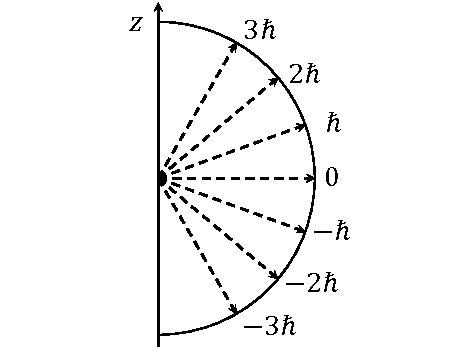
\includegraphics[height=0.9\textheight]{Seminar_06/pics/pic_01.pdf}};
\end{tikzpicture}}

\end{block}

\only<3>{
\begin{block}{Энергия}
\begin{gather*}
    \langle \hat{L_z^2}\rangle=\hbar^2\dfrac{l^2+ \dots  +(-l)^2}{2l+1} =\hbar^2\dfrac{\sum\limits_{m=-l}^{l}m^2}{2l+1} = \dfrac{\hbar^2}{3}l(l+1)\\
    \langle \hat{L^2}\rangle = \hbar^2l(l+1)
\end{gather*}
\end{block}
}


\end{frame}

\begin{frame}[t]{Более строго про энергию}
\begin{gather*}
     \hat{L^2} = -\hbar^2 \left[ \dfrac{1}{\sin{\theta}}\dfrac{\partial}{\partial\theta} \left(\sin{\theta}\dfrac{\partial}{\partial \theta}\right) + \dfrac{1}{\sin^2{\theta}}\dfrac{\partial^2}{\partial \varphi^2}\right]\\
     \hat{L^2} \psi = \langle \hat{L^2}\rangle \psi\\
     \psi = Y_{lm}(\theta; \varphi)
\end{gather*}
Здесь $Y_{lm}; n,m \in \{\mathbb{N}, 0\}$ -- специальные комплекснозначные сферические функции, которые можно посмотреть например в Ладавшице или википедии.\\

\begin{block}{Уровни энергии ротатора}
\begin{equation*}
    E_l=\dfrac{\hbar^2l(l+1)}{2I}, l\in \mathbb{N}
\end{equation*}
\end{block}
\end{frame}

\begin{frame}{Боровская теория атома водорода}\scriptsize
\only<1->{\begin{block}{Основные постулаты}
\begin{itemize}
    \item Наличие в атоме стационарных орбит, на которых электроны живут сколь угодно долго
    \item Излучение происходит только при переходе с одной орбиты на другую
    \item Момент импульса электрона квантуется
\end{itemize}
\end{block}}
\only<2>{\begin{block}{Уровни энергии}
\begin{gather*}
    \begin{cases}
     mvr = \hbar n; n\in \mathbb{N}\\[10pt]
     m\dfrac{v^2}{r} = \dfrac{Ze^2}{r}
     \end{cases}
     \Rightarrow
     \begin{cases}
     r_n = \dfrac{\hbar^2}{Ze^2m}n^2\\[10pt]
     E_n = -\dfrac{Z^2me^4}{2\hbar^2} \dfrac{1}{n^2} = -Z^2 Ry\dfrac{1}{n^2}
     \end{cases}
\end{gather*}
$Ry = 13.6$ эВ -- постоянная Ридберга
\end{block}}
\end{frame}


\begin{frame}{Строгая теория атома водорода}\scriptsize
\only<1>{\begin{block}{Уравнение Шредингера}
\begin{gather*}
    -\dfrac{\hbar^2}{2m}\Delta\psi + U(r)\psi = E\psi\\
    -\dfrac{\hbar^2}{2m}\dfrac{1}{r^2}\dfrac{\partial}{\partial r}\left( r^2 \dfrac{\partial\psi}{\partial t}\right) + U(r)\psi +\dfrac{1}{2mr^2}\hat{L^2}\psi = E\psi\\
    \psi(r, \theta, \varphi) = \dfrac{\xi(r)}{r}\times Y_{lm}(\theta; \varphi)\\
    \psi_{nlm}(r, \theta, \varphi) = A \exp{(-\varkappa_n r)}r^l\left[\sum\limits_{i=0}^{n-l-1}a_{l+1+i}r^i\right]Y_{lm}(\theta, \varphi)
\end{gather*}
\end{block}}
\only<2>{\begin{block}{Смысл}
\begin{itemize}
    \item $n = 1, 2, 3, \dots $ -- главное квантовое число. Отвечает за основной уровень энергии, чем больше, тем ближе энергия электрона к 0
    \item $l = 0, 1, 2, \dots, n-1$ -- орбитальное квантовое число. Отвечает за полный момент импульса электрона для соответствующего уровня энергии $n$. Всегда меньше главного квантового числа. Исторически также принято обозначать буквами $\{s,p,d,f, \dots \} \sim \{0,1,2,3, \dots\}$
    \item $m = -l, -l+1, \dots, l-1, l$ -- магнитное квантовое число, показывает проекцию полного момента на выделенную ось
\end{itemize}
\end{block}
\begin{block}{Сколько всего состояний}
\begin{table}[H]
\begin{tabular}{|l|l|l|l|l|l|}
\hline
\multicolumn{1}{|c|}{$n$} & \multicolumn{1}{c|}{$l$}                            & \multicolumn{1}{c|}{$m$}                                                                                            & \multicolumn{1}{c|}{Состояние}                       & \multicolumn{1}{c|}{Кратность вырождения}         & \multicolumn{1}{c|}{Всего состояний} \\ \hline
1                       & 0                                                 & 0                                                                                                                 & 1S                                                   & 1                                                 & 1                                    \\ \hline
2                       & \begin{tabular}[c]{@{}l@{}}0 \\ 1\end{tabular}    & \begin{tabular}[c]{@{}l@{}}0\\ 0, $\pm$ 1\end{tabular}                                               & \begin{tabular}[c]{@{}l@{}}2S\\ 2P\end{tabular}      & \begin{tabular}[c]{@{}l@{}}1\\ 3\end{tabular}     & 4                                    \\ \hline
3                       & \begin{tabular}[c]{@{}l@{}}0\\ 1\\ 2\end{tabular} & \begin{tabular}[c]{@{}l@{}}0\\ 0,$\pm$ 1\\ 0,$\pm$ 1, $\pm$ 2\end{tabular} & \begin{tabular}[c]{@{}l@{}}3S\\ 3P\\ 3D\end{tabular} & \begin{tabular}[c]{@{}l@{}}1\\ 3\\ 5\end{tabular} & 9                                    \\ \hline
\end{tabular}
\end{table}
\end{block}
}

\only<3>{
\begin{block}{Орбитали}
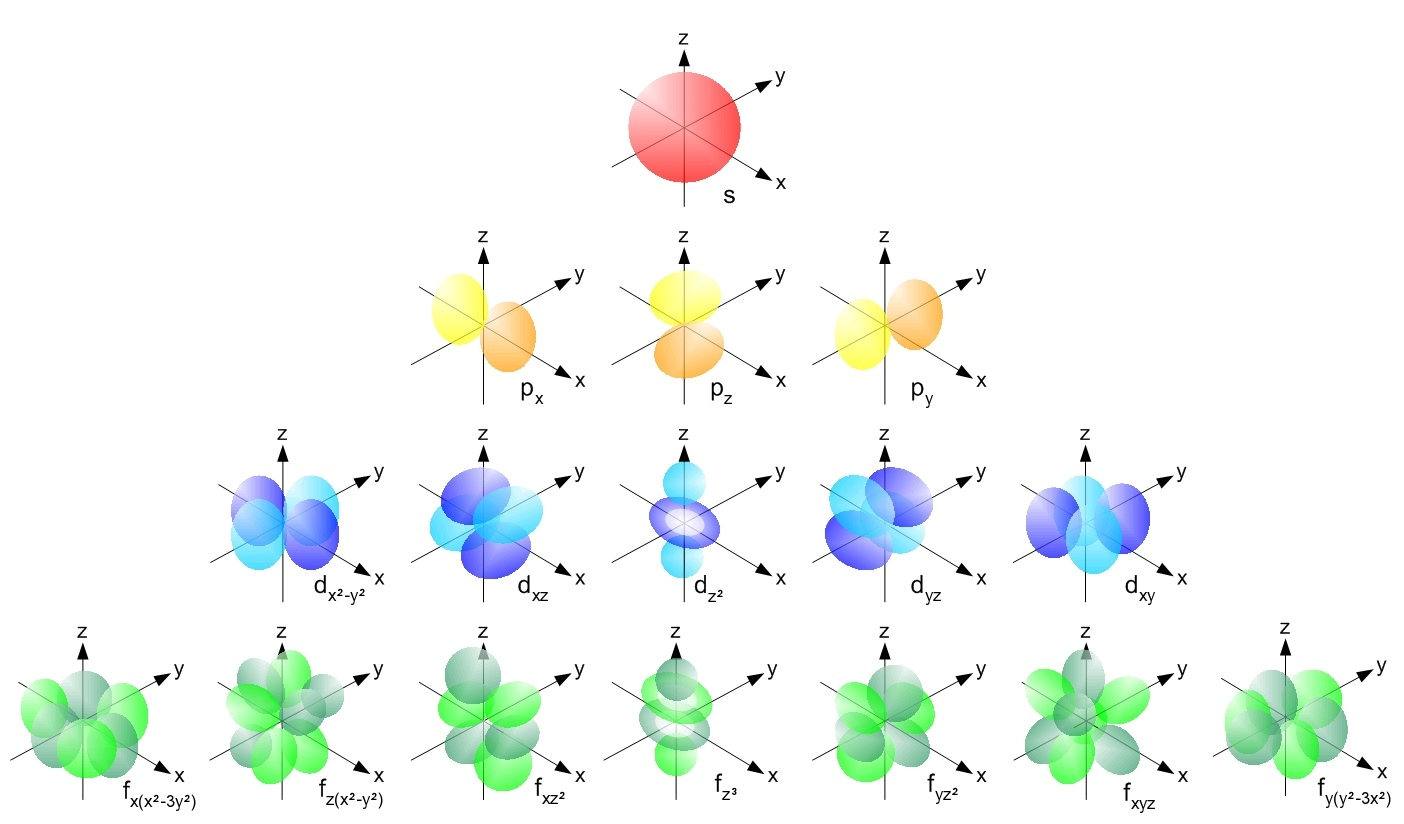
\includegraphics[width=0.97\textwidth,height=\textheight,keepaspectratio]{Seminar_06/pics/Pic_03.jpg}
\end{block}
}
\end{frame}

\begin{frame}{комментарии и добавки}\scriptsize
\begin{block}{Неверность боровской теории}
Совпадение уровней энергии:
\begin{equation*}
   E_n = -\dfrac{Z^2me^4}{2\hbar^2} \dfrac{1}{n^2} = -Z^2 Ry\dfrac{1}{n^2}
\end{equation*}
Несовпадение момента импульса!
\end{block}
\begin{block}{Поправка к постоянной Ридберга}
\begin{equation*}
    R=\dfrac{Ry}{1+m/M_{\text{яд}}}
\end{equation*}
\end{block}

\end{frame}


\begin{frame}{Задача 4.7}\scriptsize
\only<1>{\begin{block}{Условие}
Найти среднее расстояние электрона от ядра в 1s-состоянии в атоме водорода. Волновая функция основного состояния $\psi_{100}(r, \theta, \varphi) = \dfrac{1}{\sqrt{\pi r_1^3}}\exp{\left(-\dfrac{r}{r_1} \right)}$, $r_1$ -- радиус первой Боровской орбиты.
\end{block}}
\only<2>{\begin{block}{Решение}
Эта задача является по сути отсылкой к прошлому семинару. Тут нам дана волновая функция, надо найти среднее значение оператора координаты, проинтегрировав во всему пространству с учетом сферической симметрии:
\begin{equation*}
    \langle r\rangle = \int\limits_0^{\infty} \psi^*_{100} r \psi_{100} 4\pi r^2 dr =\dfrac{1}{\pi r_1^3}\int\limits_0^{\infty} \exp{\left(- \dfrac{2r}{r_1} \right)} r^3 dr = \dfrac{3}{2}r_1
\end{equation*}

\end{block}}
\end{frame}

\begin{frame}{Задача 4.29}\scriptsize
\only<1>{\begin{block}{Условие}
В 1989 году в ЦЕНРе при пропускании медленных антипротонов через водородную камеру наблюдалось образование протонимума -- атома, состоящего из протона и антипротона. Энергия излучения, соответствующая переходу протониума из состояния 2p в состояние 1s оказалась равной 10.1 кэВ. Определить вклад сильного взаимодействия в разность энергии указанных уровней.
\end{block}}
\only<2>{\begin{block}{Решение}
Если учесть движение протонов друг относительно друга:
\begin{equation*}
    E_n = - \dfrac{Ry}{1+m_e/m_p}\dfrac{1}{n^2} = -Ry\dfrac{m_p}{2m_e} \dfrac{1}{n^2} = -\dfrac{12.5}{n^2} \text{ кэВ}
\end{equation*}
У нас переход с $n=2$ на $n=1$
\begin{equation*}
    \Delta E = 12.5\left(\dfrac{1}{1^2} - \dfrac{1}{2^2}\right) = 9.4 \text{ кэВ}
\end{equation*}
Полученный результат не совпадает с экспериментальным из-за того, что в наших расчетах мы использовали только потенциал кулоновского взаимодействия, но ведь есть еще и другие, которые могут оказаться существенными. Величина этого несовпадения $\delta E = 10.1 - 9.4 = 0.7$ кэВ. Именно это и есть вклад сильного взаимодействия. 
\end{block}}
\end{frame}

\begin{frame}{Задача 5.11}\scriptsize
\only<1>{\begin{block}{Условие}
В опытах с равными молекулами измерялись энергии перехода между тремя последовательными уровнями энергии вращательной полосы двухатомной молекулы. Найти
квантовые числа $l$ этих уровней и момент инерции $I$ молекулы в этих случаях.
\begin{figure}[h]
    \centering
    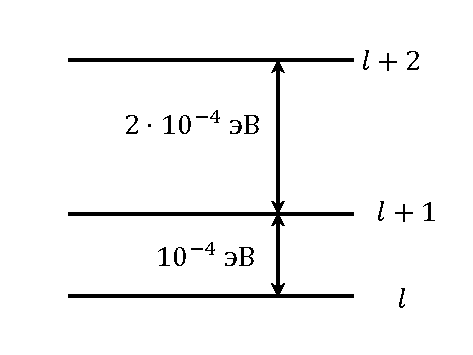
\includegraphics[width=0.5\textwidth,height=\textheight,keepaspectratio]{Seminar_06/pics/pic_04.pdf}
\end{figure}
\end{block}}
\only<2>{\begin{block}{Решение}
Поскольку уровни энергии последовательный, они соответствуют уровням с номерами $l, l+1, l+2$, а тогда сама энергия будет пропорциональная $l(l+1), (l+1)(l+2), (l+2)(l+3)$. Из соотношения энергии между уровней найдем $l$:
\begin{equation*}
    \dfrac{2}{1} = \dfrac{(l+2)(l+3)-(l+1)(l+2)}{(l+1)(l+2)-l(l+1)} = \dfrac{l+2}{l+1} \Rightarrow l=0
\end{equation*}
Для нахождения момента инерции воспользуемся данными оп переходе с $l=0$ на $l=1$:
\begin{gather*}
    \Delta E_{0\rightarrow 1} = \dfrac{\hbar^2 l(l+1)}{2I}\\
    I = \dfrac{\hbar^2}{\Delta E_{0\rightarrow 1}} = 6.9\cdot 10^{-39} \text{ г}\cdot\text{см}^2
\end{gather*}
\end{block}}
\end{frame}

\begin{frame}{Задача 5.13}\scriptsize
\only<1>{\begin{block}{Условие}
Какова максимальная длина волны СВЧ-излучения, с помощью которой можно вызвать переход между ротационными уровнями молекул хлорa? Расстояние между ядрами атомов в молекуле $\text{Cl}_2$ равно $d = 2 \cdot 10^{−8}$ см. Относительная атомная масса изотопа хлора $A=35$.
\end{block}}
\only<2>{\begin{block}{Решение}
Максимальная длина волны, соответствует минимальной частоте, и, как следствие минимальной энергии перехода. А она будет как раз между 0 и 1 уровнями (мы увидели это в предыдущей задаче). Осталось вспомнить как посчитать момент инерции, чтобы подставить в формулу для энергии. Для двухатомных молекул все просто: $I = \mu d^2$, где $\mu$ -- приведенная масса этой молекулы. В нашем случае, она равна $m_{\text{Cl}}/2 = 35/2 \cdot 1.6 \cdot 10^{-24}$ г, так как атомы в молекуле одинаковые. Теперь выразим максимальную длину волны из формулы для энергии:
\begin{equation*}
    \lambda = \dfrac{2\pi \hbar с m_{\text{Cl}} d^2}{2\hbar^2} = 2.1 \text{ см}
\end{equation*}
\end{block}}
\end{frame}

\begin{frame}{Задача 5.25}\scriptsize
\only<1>{\begin{block}{Условие}
В угарном газе из-за возбуждения колебаний молекул наблюдается  пик поглощения инфракрасного излучения на длине волны $\lambda = 4.61$ мкм. Оценить амплитуду нулевых колебаний в молекуле угарного газа. Оценить температуру, при которой амплитуда тепловых колебаний превзойдет ее.
\end{block}}
\only<2>{\begin{block}{Решение}
Энергия у осциллятора не бывает равна нулю из-за соотношения неопределнностей, и такая молекула колеблется с известной нам энергией $\hbar \omega/2$. Тогда мы можем записать эту энергию через коэффициент жесткости и амплитуду нулевых колебаний, а коэффициент жесткости выразить через частоту и приведенную массу:
\begin{gather*}
    \begin{cases}
       \dfrac{\hbar \omega}{2} = \dfrac{kA_0^2}{2}\\
       \omega^2 = \dfrac{k}{\mu}
    \end{cases} \Rightarrow A_0 = \sqrt{\dfrac{\hbar}{\mu \omega}} = 4.74\cdot 10^{-10} \text{ см}
\end{gather*}
Условие на температуру получается из сравнения энергии нулевых колебаний и характерной тепловой энергии:
\begin{equation*}
    kT = \dfrac{\hbar \omega}{2} \Rightarrow T\sim 3100 \text{ К}
\end{equation*}
\end{block}}
\end{frame}



\begin{frame}[t]{Комментарии к задачам из задания}\scriptsize
\begin{itemize}
\item Задача 4.29 Решена 
\item Задача 4.38 Задача на закон Мозли и экранирование, решена в задачнике.
\item Задача 4.42 Очень похожа на 4.41, решенную в задачнике
\item Задача 4.45 Оценить радиус орбиты мюона и подумать, как это может повлиять на решение. 
\item Задача 5.16 Задача почти что обратная к 5.13
\item Задача 5.25 Решена
\item Задача 5.51 Для разных изотопов будет немного разная приведенная масса, и соответственно момент инерции. Далее стандартные уровни энергии для ротатора
\item Задача 5.55 Дублирую указание из учебника. Энергия, как функция уровня, должна расти монотонно. 
\end{itemize}
\end{frame}

\end{document}